\documentclass{llncs}
\usepackage[dvips,final]{graphics}
\usepackage{amsmath}
\usepackage{times}
%
%
%
\begin{document}
\mainmatter

%
\title{An Image Inpainting Technique based on the Fast Marching Method}
\titlerunning{An Image Inpainting Technique}
\author{Alexandru Telea}

\authorrunning{Alexandru Telea}
\tocauthor{Alexandru Telea (Eindhoven University of Technology)}

\institute{Department of Mathematics and Computer Science,\\
Eindhoven University of Technology, \\
Den Dolech 2,Eindhoven 5600 MB, The Netherlands, \\
\email{alext@win.tue.nl},
\texttt{http://www.win.tue.nl/$\sim$alext}}
%
%
\maketitle
%
%
\begin{abstract} 
% 
  Digital inpainting provides a means for reconstruction of small
damaged portions of an image. Although the inpainting basics are
straightforward, most inpainting techniques published in
the literature are complex to understand and implement.
We present here a new algorithm for digital inpainting based on the fast
marching method for level set applications. Our algorithm is very
simple to implement, is fast, and produces nearly identical results as
more complex, and usually slower, known methods. Source code is available online.
\end{abstract}
%
%
\section{Introduction}
%
%
 Digital inpainting, the technique of reconstructing small damaged portions
of an image, has received considerable attention in the last years.
Digital inpainting serves a wide range of
applications, such as removing text and logos from still images or videos, reconstructing
scans of deteriorated images by removing scratches or stains, or creating
artistic effects.
 Most inpainting methods work as follows. First, the
image regions to be inpainted are selected, usually in a
manual way. Next, color information is propagated inwards from the region
boundaries, i.e. the known image information is used to fill-in the missing areas. 
In order to produce a perceptually plausible reconstruction, an inpainting
technique should attempt to continue the 
\textit{isophotes} (lines of equal gray value) as smoothly as possible inside the
reconstructed region. In other words, the missing region should be inpainted
such that the inpainted gray value and gradient extrapolate
the gray value and gradient outside this region. 
  
Several inpainting methods are based on the above ideas.
In \cite{bertalmio1,bertalmio2}, the image smoothness
information, estimated by the image Laplacian, is propagated along the
isophotes directions, estimated by the image gradient rotated with 90
degrees. The \textit{Total Variational} (TV) model~\cite{chan} uses an
Euler-Lagrange equation coupled with anisotropic diffusion to maintain the
isophotes' directions. The \textit{Curvature-Driven Diffusion} (CCD)
model~\cite{chan2} enhances the TV method to drive diffusion along the isophotes' directions
and thus allows inpainting thicker regions. All above methods essentially 
solve a partial differential equation (PDE) that describes
the color propagation inside the missing region, subject to various
heuristics that attempt to preserve the
isophotes' directions. Preserving isophotes is, however desirable, never
perfectly attained in practice. The main problem is that both isophote
estimation and information propagation are subject to numerical diffusion.
Diffusion is desirable as it stabilizes the PDEs to be solved, but leads
inevitably to a cetain amount of blurring of the inpainted area.

A second type of methods~\cite{oliveira}
repeatedly convolves a simple 3x3 filter over the missing regions to
diffuse known image information to the missing pixels.
  
However impressive, the above methods have several drawbacks that preclude
their direct use in practice. The PDE-based methods require implementing non-trivial iterative numerical
methods and techniques, such as anisotropic diffusion and multiresolution schemes \cite{bertalmio1}.
Little or no information is given on practical implementation details such as various thresholds or
discretization methods, although some steps are mentioned as numerically unstable.
Moreover, such methods are quite slow, e.g. a few minutes for the relatively
small inpainting region shown in Fig.~\ref{fig:example3}.
In contrast, the convolution-based method described in~\cite{oliveira} 
is simple to implement and fast. However, this method has no provisions for
preserving the isophotes' directions.
High-gradient image areas must be manually selected before inpainting and
separately treated in order not to be blurred. 

  We propose a new inpainting algorithm based on propagating an image smoothness estimator along the
image gradient, similarly to~\cite{bertalmio1}. We estimate the image
smoothness as a weighted average over a known image neighborhood of the pixel to
inpaint. We treat the missing regions as level sets and use
the fast marching method (FMM) described in~\cite{sethian} to propagate the
image information. Our approach has several advantages:
\begin{itemize}
  \item it is very simple to implement (the complete pseudocode is given here).
  \item it is considerably faster than other inpainting methods
       --- processing an 800x600 image (Fig.~\ref{fig:example3}) takes under 3 seconds on a 800 MHz PC.
  \item it produces very similar results as compared to the other methods.
  \item it can easily be customized to use different local inpainting strategies.
\end{itemize}
%
%
 In Section~\ref{sec:method}, we describe our method. Section~\ref{sec:discussion}
presents several results, details our method's advantages and limitations
in comparison to other methods, and discusses possible enhancements. Source
code of a sample method implementation is available online at the address
listed at the end of the paper.
%
%
	\begin{figure}[h] \centering
	\resizebox{1.0\textwidth}{!}{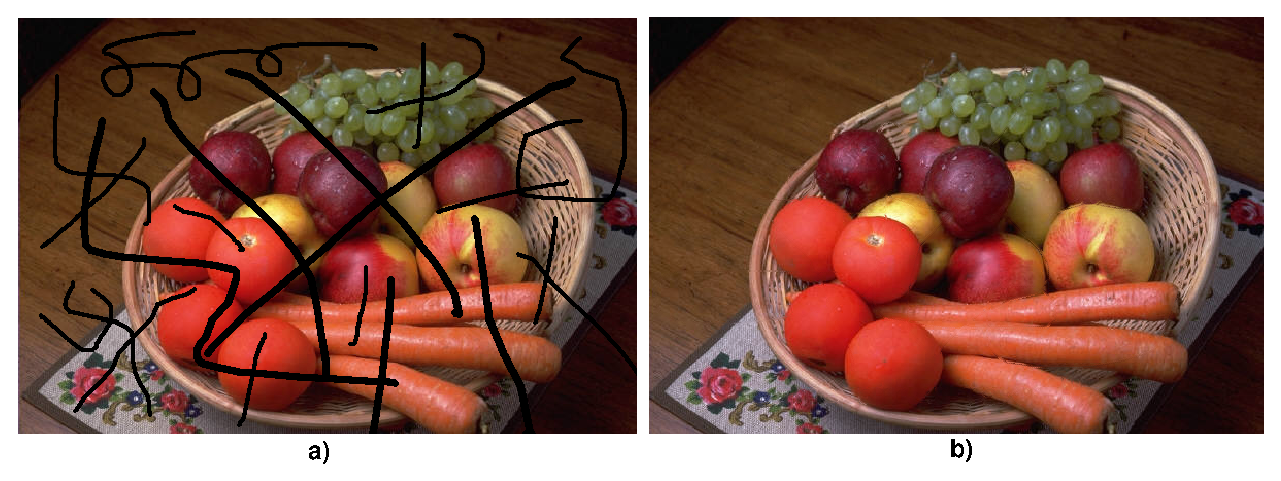
\includegraphics{EPS/example3.eps}}
	\caption{800x600 image inpainted in under 3 seconds}
	\label{fig:example3} 
        \end{figure} 
%
%   
%
%
\section{Method}
\label{sec:method}
%
This section describes our inpainting method. First,
we introduce the mathematical model we base our inpainting
on (Sec.~\ref{sec:model}). Next, we describe how the missing regions are
inpainted using the FMM (Sec.~\ref{sec:fmm}). Finally, we detail the
implementation of inpainting one point on the missing region's boundary
(Sec.~\ref{sec:inp_function}).
%
\subsection{Mathematical model}
\label{sec:model}
%
 To explain our method, consider Fig.~\ref{fig:method}, in which one must
inpaint the point $p$ situated on the boundary $\partial\Omega$ of the
region to inpaint $\Omega$. Take a small neighborhood $B_{\varepsilon}(p)$
of size $\varepsilon$ of the known image around $p$
(Fig.~\ref{fig:method}~a). As described in~\cite{bertalmio1,oliveira,chan},
the inpainting of $p$ should be determined by the values
of the known image points close to $p$, i.e. in $B_{\varepsilon}(p)$. 
We first consider gray value images, color images being a natural extension (see Sec.~\ref{sec:implem}).
%
	\begin{figure}[h] \centering
	\resizebox{0.65\textwidth}{!}{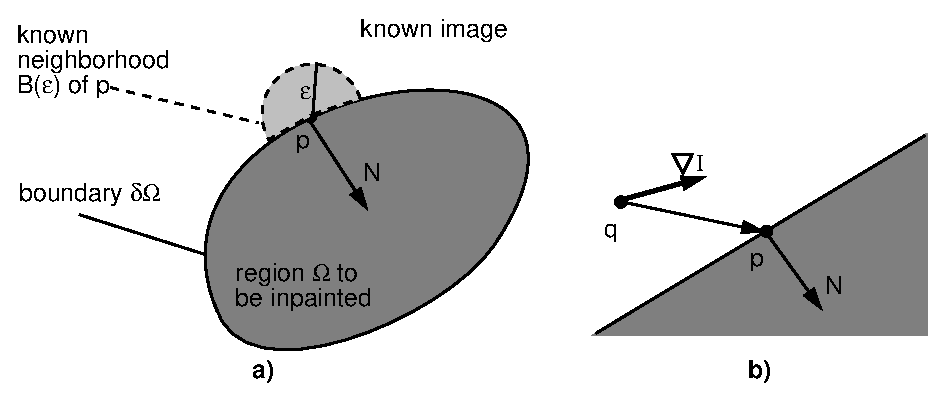
\includegraphics{EPS/method.eps}}
	\caption{The inpainting principle}
	\label{fig:method} 
        \end{figure} 
%
For $\varepsilon$ small enough, we consider a first order approximation $I_q(p)$
of the image in point $p$, given the image $I(q)$ and gradient $\nabla I(q)$
values of point $q$ (Fig~\ref{fig:method}~b):
%
%
\begin{equation}
   I_q(p) = I(q) + \nabla I(q) (p-q)
\label{eqn:linear}
\end{equation}
%
%
Next, we inpaint point $p$ as function of all points $q$ in
$B_{\varepsilon}(p)$ by summing the estimates of all points $q$, 
weighted by a normalized weighting function $w(p,q)$:
%
%
\begin{equation}
  I(p) = \frac{\sum_{q \in B_{\varepsilon}(p)} w(p,q) [I(q) + \nabla I(q) (p-q)]}
              {\sum_{q \in B_{\varepsilon}(p)} w(p,q)}
\label{eqn:sum}
\end{equation}
%
%
The weighting function $w(p,q)$, detailed in Sec.~\ref{sec:inp_function}, 
is designed such that the inpainting of $p$ propagates the gray value as well 
as the sharp details of the image over $B_{\varepsilon}(p)$. 
%
\subsection{Adding inpainting to the FMM}
\label{sec:fmm}
%
%
 Section~\ref{sec:model} explained how to inpaint
a point on the unknown region's boundary $\partial\Omega$ as a function of
known image pixels only. To inpaint the whole $\Omega$, we iteratively apply
iteratively apply Equation~\ref{eqn:sum} to all the discrete pixels of
$\partial\Omega$, in increasing distance from $\partial\Omega$'s initial
position $\partial\Omega_i$, and advance the boundary inside $\Omega$ until the whole
regions has been inpainted (see pseudocode in Fig.~\ref{fig:pseudo}). 
Inpainting points in increasing
distance order from $\partial\Omega_i$ ensures that areas closest to known
image points are filled in first, thus mimicking manual inpainting
techniques~\cite{bertalmio1,bertalmio2}. 
%
	\begin{figure}[h] \centering
	\resizebox{0.45\textwidth}{!}{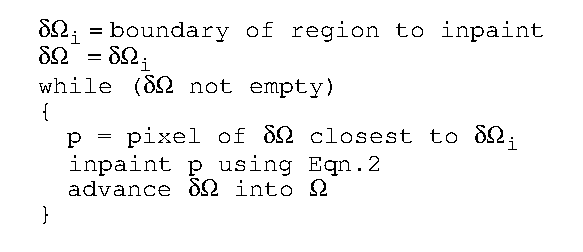
\includegraphics{EPS/pseudo.eps}}
	\caption{Inpainting algorithm}
	\label{fig:pseudo} 
        \end{figure} 
%

Implementing the above requires thus a method that propagates
$\partial\Omega$ into $\Omega$ by advancing the pixels of $\partial\Omega$
in order of their distance to the initial boundary $\partial\Omega_i$. 
For this, we use the fast marching method (FMM) developed by Sethian et al.
\cite{sethian}. In brief, the FMM is an algorithm that solves the Eikonal equation:
%
%
\begin{equation}
   |\nabla T| = 1 \mbox{~~~~~on $\Omega$,~~~~~with $T=0$ on $\partial\Omega$}
\label{eqn:eikonal}
\end{equation}
%
The solution $T$ of Eqn.~\ref{eqn:eikonal} is the distance map of the $\Omega$ pixels to the boundary
$\partial\Omega$. The level sets, or isolines, of $T$ 
are exactly the successive boundaries $\partial\Omega$ of the shrinking
$\Omega$ that we need for inpainting. The normal $N$ to
$\partial\Omega$, also needed for inpainting, is exactly $\nabla T$. The FMM
guarantees that pixels of $\partial\Omega$ are always processed in
increasing order of their distance-to-boundary $T$~\cite{fmm_book}, i.e.
that we always inpaint the closest pixels to the known image area first. 

We prefer the FMM over other 'distance transform' (DT) methods that compute the distance map $T$ to a boundary $\partial\Omega$
(e.g.~\cite{chamfer1,chamfer2,roerdinck}). The FMM's main advantage is that it
\textit{explicit} maintains the narrowband that
separates the known from the unknown image area \textit{and} specifies which is the next pixel to
inpaint. Other DT methods compute the distance map $T$ but do not maintain an
explicit narrowband. Adding a narrowband structure to these method would
complicate their implementation, whereas the FMM provides this structure by
default.

To explain in detail our use of the FMM  --- and since the FMM is not
straightforward to implement from the reference
literature~\cite{sethian,fmm_book} --- we provide next its complete pseudocode. 
  The FMM maintains a so-called \textit{narrow band} of pixels, which is
exactly our inpainting boundary $\partial\Omega$. For every image pixel, we store
its value $T$, its image gray value $I$ (both represented as floating-point
values),  and a flag $f$ that may have three values:
\begin{itemize}
  \item\textit{BAND}: the pixel belongs to the narrow band. Its $T$ value
  undergoes update.
  \item\textit{KNOWN}: the pixel is outside $\partial\Omega$, in the known
  image area. Its $T$ and $I$ values are known.
  \item\textit{INSIDE}: the pixel is inside $\partial\Omega$, in the region to inpaint. Its $T$
  and $I$ values are not yet known.
\end{itemize}
%
%
  The FMM has an initialization and propagation phase, as follows.
First, we set $T$ to zero on and outside the boundary
$\partial\Omega$ of the region to inpaint and to some large value (in practice $10^6$)
inside, and initialize $f$ over the whole image as explained
above. All $BAND$ points are inserted in a heap \texttt{NarrowBand}
sorted in ascending order of their $T$ values. 
Next, we propagate the $T$, $f$, and $I$ values using the code
shown in Fig.~\ref{fig:fmm_code}.
%
	\begin{figure}[h] \centering
	\resizebox{0.75\textwidth}{!}{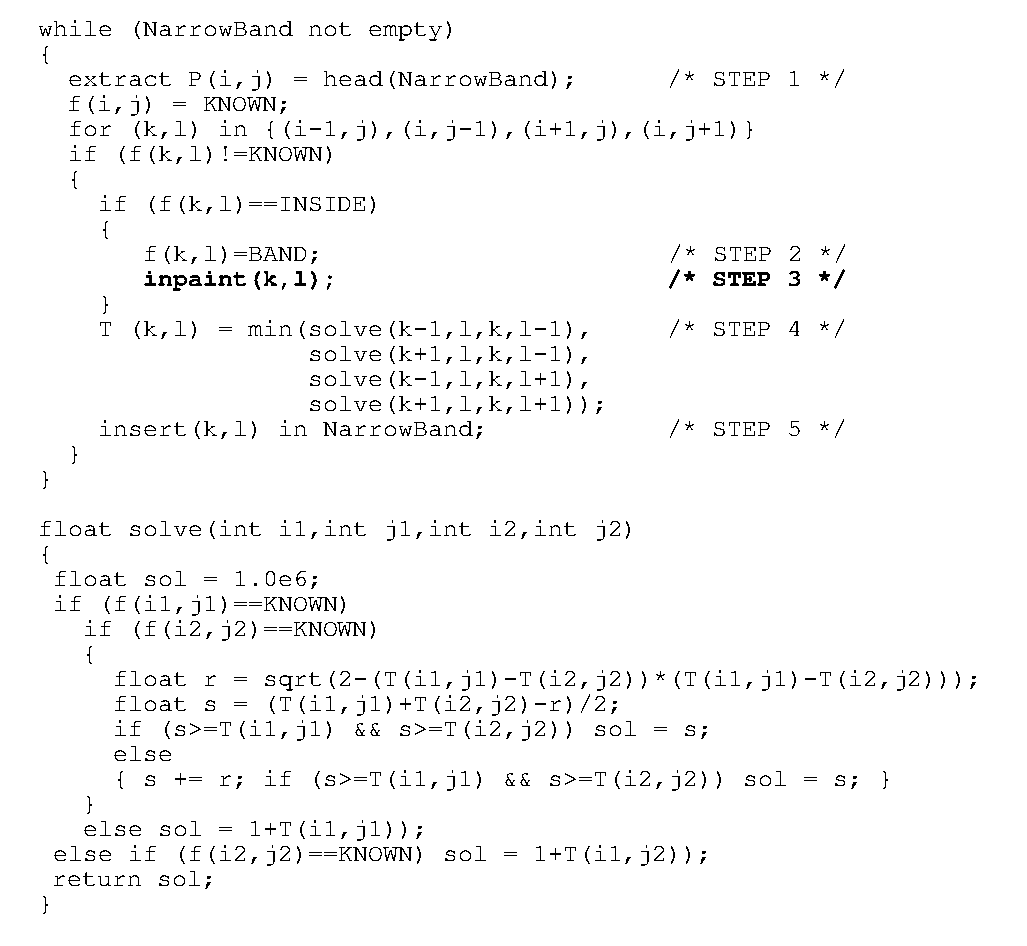
\includegraphics{EPS/code.eps}}
	\caption{Fast marching method used for inpainting}
	\label{fig:fmm_code} 
        \end{figure} 
%
%
Step 1 extracts the $BAND$ point with the smallest $T$. Step 2 marches
the boundary inwards by adding new points to it. Step 3 performs the
inpainting (see Sec.~\ref{sec:inp_function}). Step 4 propagates the value
$T$ of point $(i,j)$ to its neighbors $(k,l)$ by solving the finite difference discretization of
Eqn.~\ref{eqn:eikonal} given by:
%
\begin{equation}
  \mbox{max}(D^{-x}T,-D^{+x}T,0)^2+\mbox{max}(D^{-y}T,-D^{+y}T,0)^2 = 1
\label{eqn:quad}
\end{equation}
%
where $D^{-x}T(i,j) = T(i,j)-T(i-1,j)$ and $D^{+x}T(i,j) = T(i+1,j)-T(i,j)$
and similarly for $y$. Following the upwind idea of Sethian~\cite{sethian},
we solve Eqn.~\ref{eqn:quad} for $(k,l)$'s four quadrants and retain
the smallest solution. Finally, step 5 (re)inserts $(k,l)$
with its new $T$ in the heap.

%
%
\subsection{Inpainting one point}   
\label{sec:inp_function}
%
%
We consider now how to inpaint a newly discovered point $(k,l)$, as function of the
$KNOWN$ points around it, following the idea described in Sec.~\ref{sec:model}
(step 3 in Fig.~\ref{fig:fmm_code}, detailed in Fig.~\ref{fig:inpaint_code})).
%
	\begin{figure}[h] \centering
	\resizebox{0.7\textwidth}{!}{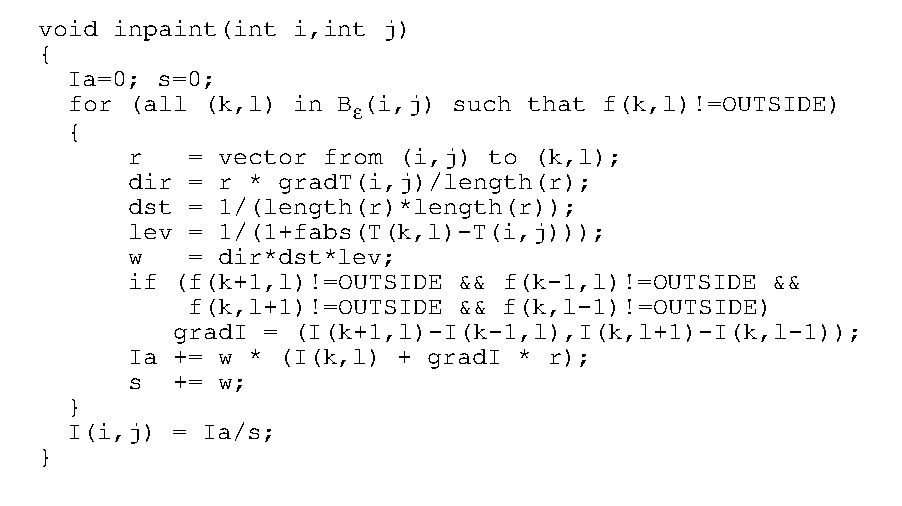
\includegraphics{EPS/inpaint_code.eps}}
	\caption{Inpainting one point}
	\label{fig:inpaint_code} 
        \end{figure} 
%
We iterate over the $KNOWN$ points in the neighborhood $B_{\varepsilon}$ of
the current point $(i,j)$ and compute $I(i,j)$ following
Eqn.~\ref{eqn:sum}. The image gradient $\nabla I$ (\texttt{gradI} in the
code) is estimated by central differences. As stated in Sec.~\ref{sec:model}, the design of the
weighting function $w(p,q)$ is crucial to propagate the sharp image details and the smooth
zones as such into the inpainted zone. We design $w(p,q) = dir(p,q) \cdot
dst(p,q) \cdot lev(p,q)$ as a product of three factors:
%
%
%\begin{equation}
%  w(p,q)=dir(p,q) \cdot dst(p,q) \cdot lev(p,q)
%\end{equation}
%
%
\begin{eqnarray*}
  dir(p,q) &=& \frac{p-q}{||p-q||} \cdot N(p)\\
  dst(p,q) &=& \frac{d_0^2}{||p-q||^2} \\
  lev(p,q) &=& \frac{T_0}{1+|T(p)-T(q)|}  
\end{eqnarray*}
%
%
The \textit{directional} component $dir(p,q)$ ensures that the
contribution of the pixels close to the normal direction
$N=\nabla T$ (\texttt{gradT} in the code), i.e. close to the
FMM's information propagation direction, is higher than for those further from
$N$. The \textit{geometric distance} component $dst(p,q)$ decreases the
contribution of the pixels geometrically farther from $p$.  
The \textit{level set} distance
component $lev(p,q)$ ensures that pixels close to the contour
through $p$ contribute more than further pixels. Both $dst$ and $lev$ are
relative with respect to the reference distances $d_0$ and $T_0$. In practice, we set
$d_0$ and $T_0$ to the inter-pixel distance, i.e. to 1.
Overall, the above factors model the manual inpainting heuristics~\cite{bertalmio1} that
describe how to paint a point by strokes bringing color from a small region
around it.

For $\varepsilon$ up to about
6 pixels, i.e. when inpainting thin regions, $dst$ and $lev$ have
a weak effect. For thicker regions to inpaint, such as
Fig.~\ref{fig:example2}~d where we used an $\varepsilon$ of 12 pixels, 
using $dst$ and $lev$ provides better
results than using $dir$ alone. The above is clearly visible in
Fig.~\ref{fig:ellipse}, on a test image taken from~\cite{bertalmio1},  where
the missing ring shaped region is over 30 pixels thick.
Figure~\ref{fig:ellipse}~c shows, on an image detail, the effect of $dir$ alone. The results are
somewhat less blurry when $dir$ and $dst$ (Fig.~\ref{fig:ellipse}~d) or
$dir$ and $lev$ (Fig.~\ref{fig:ellipse}~e) are used together. The inpainting
is visually the best when all three components are used (Fig.~\ref{fig:ellipse}~f).
%
%
	\begin{figure}[h] \centering
	\resizebox{0.81\textwidth}{!}{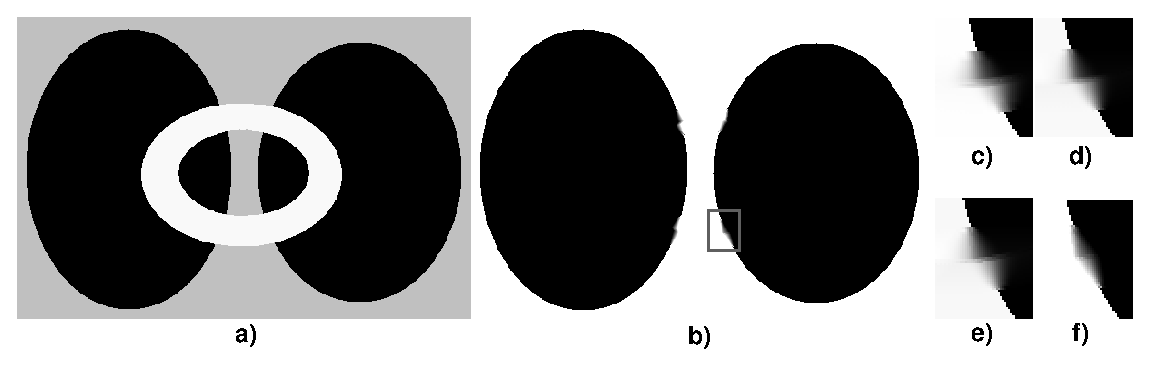
\includegraphics{EPS/ellipse.eps}}
	\caption{Thick region to inpaint (a) and result (b). Effect of weighting functions: 
         direction (c), direction and geometric distance (d), direction and level set distance (e),
         direction, geometric, and level set distance (f)}
	\label{fig:ellipse} 
        \end{figure} 
%
%
%
%
\subsection{Implementation details}
\label{sec:implem}
%
%
  Several implementation details are important. First, we compute the
boundary normal $N=\nabla T$ by numerical derivation of the field $T$
computed by the FMM. Derivating $T$ on the fly as it is computed by the
FMM is unstable, since we are not guaranteed that a large enough
neighborhood around the current point contains only $KNOWN$ points.
We first run the FMM outside the initial inpainting boundary
$\partial\Omega$ and obtain the distance field $T_{out}$. Since we use only
those points closer to $\partial\Omega$ than $\varepsilon$, we run the FMM
outside $\partial\Omega$ only until we reach $T > \varepsilon$. This
restricts the FMM computations to a band of thickness $\varepsilon$ around
$\partial\Omega$, thus speeding up the process. Next, we run the FMM
inside $\partial\Omega$ and obtain $T_{in}$. The field $T$ over the whole
image is given by:
%
\begin{equation}
T(p) = \left\{
      \begin{array}{rcl}
      &T_{in}&(p)~~~\mbox{if}~p \in \Omega\\
      -&T_{out}&(p)~~~\mbox{if}~p \notin \Omega.
\end{array}
\right.
\end{equation}
%
Next, we smooth $T$ by a 3x3 tent filter, and then compute $\nabla T$ by
central differences. 

  The value of $\varepsilon$ giving the size of $B$ usually ranges from 3 to 10
pixels. This corresponds with the 'thickness' of the regions to inpaint,
which is usually less than 15 pixels. Higher values blur the sharp details
to be reconstructed by inpainting, although they are useful when inpainting
thicker regions. 

  The test \texttt{f(k,l)!=OUTSIDE} in Fig.~\ref{fig:inpaint_code} that
restricts $B_{\varepsilon}$ to the known image points can be changed to
\texttt{f(k,l)==KNOWN}. The results are visually identical, as
$B_{\varepsilon}$ contains very few $BAND$ pixels. However, one would use the second test
if the initial $\partial\Omega$ corresponds to unknown image pixels.

The \texttt{NarrowBand} sorted heap (Sec.~\ref{sec:fmm}) is straightforwardly implemented using
the C++ STL \texttt{multimap} container~\cite{stl}. Finally, for color (RGB) images we apply the presented 
method separately for each color channel.
%
\section{Discussion}
\label{sec:discussion}
%
%
   We have compared our inpainting method with the methods presented
by Bertalmio et al. in~\cite{bertalmio1} and Oliveira et al. in~\cite{oliveira}, further denoted by
BSCB and OBMC, by running it on the same input images (see Figures~\ref{fig:example1}
and~\ref{fig:example2}~a-c). For BSCB we used the implementation publicly available
at~\cite{implem}, whereas we reimplemented OBMC ourselves. 
Our method produced visually nearly identical results with BSCB. Compare, for example, the
inpaintings in Fig.~\ref{fig:example1}~c,d (Fig.~\ref{fig:example1}~e,f in
detail) and Fig.~\ref{fig:example2}~b,c (Fig.~\ref{fig:example2}~g,h in detail).
In contrast, the results of OBMC (shown in~\cite{oliveira}) 
were visibly more blurry for regions thicker than 6 pixels. 
%
	\begin{figure}[h] \centering
	\resizebox{1.05\textwidth}{!}{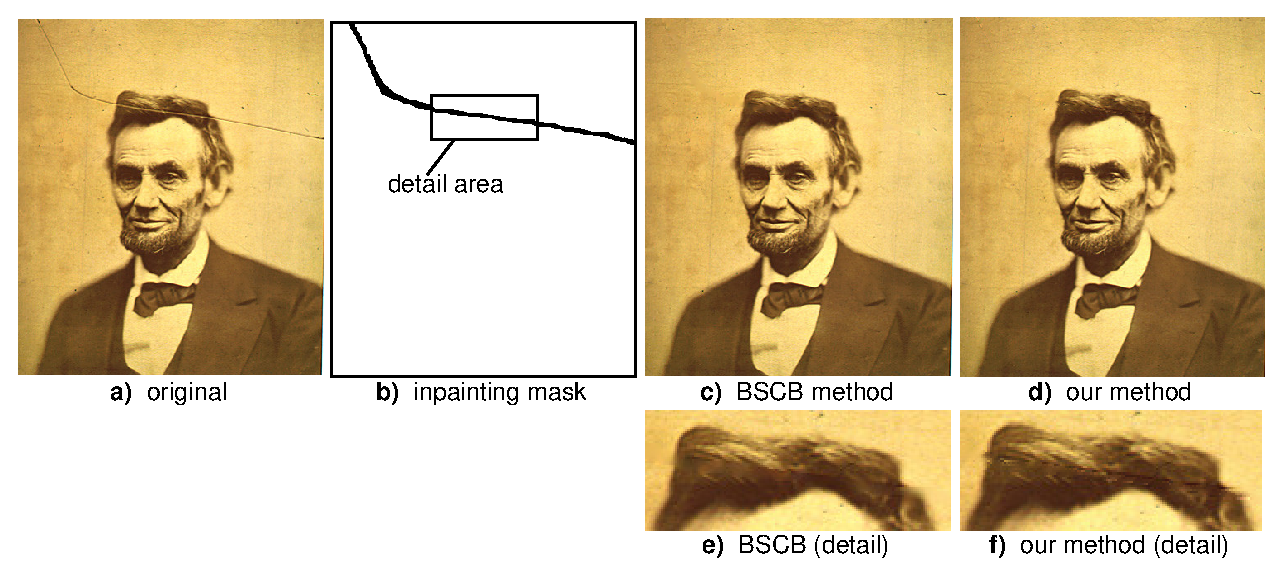
\includegraphics{EPS/example1.eps}}
	\caption{Lincoln 'cracked photo' inpainting}
	\label{fig:example1} 
        \end{figure} 
%
%   
  The running time for our method was in all cases much lower than for
BSCB. Our C++ implementation took under 3 seconds on an 800 MHz PC for a 800x600
color image with about 15\% pixels to inpaint (Fig.~\ref{fig:example3}).
On the same input, the original BSCB method, published in~\cite{bertalmio1}, is reported to take under 5 minutes on a
300 MHz PC. The BSCB implementation we used~\cite{implem}, which is
however mentioned to be unoptimized by its authors, took between 2.5 and 3 minutes on the 800
MHz PC, depending on its various parameter settings.
In contrast, OBMC takes in all cases about the same time as our method.
The above matches the fact that both OBMC and our method are linear
in the inpainted region's size. 

The main limitation of our method (applicable to the methods BSCB and
OBMC mentioned here too) is the blurring produced when inpainting
regions thicker than 10-15 pixels, especially visible when sharp isophotes
intersect the region's boundary almost tangentially. See for example the
inpainting in Fig.~\ref{fig:example2}~d,e (in
detail in Fig.~\ref{fig:example2}~i,j). The above is caused by the linear
and local character of our method. Techniques using an explicit nonlinear
and/or global image model, such as the TV~\cite{chan} and the CDD~\cite{chan2} methods,
achieve better results, at the cost of considerably more complex implementations.
%
	\begin{figure}[h] \centering
	\resizebox{1.05\textwidth}{!}{\includegraphics{EPS/example2.eps}}
	\caption{Inpainting examples. Damaged photo (a), inpainting by method BSCB (b), 
         our method (c), and close-ups (f,g,h).
         Damaged photo (d), distance-weighted inpainting (e), and close-ups (i,j)}.
	\label{fig:example2} 
        \end{figure} 

Overall, the presented inpainting method is simple to implement (our complete C++ code is 
about 500 lines), is fast, and easy to customize for different inpainting strategies.
We plan to extend the method by developing new inpainting functions that
are better able to preserve the isophotes' directions. One such way is to
integrate anisotropic diffusion, e.g. following~\cite{bertalmio1}, in the FMM boundary
evolution in order to reduce the blurring for inpainting thick regions. A
second extension would be to modulate the evolution speed of the FMM, now
equal to 1, by the image anisotropy, i.e. let inpainting 'work more' on the
high detail areas than on the smooth regions.
%
%
\section*{Acknowledgements}
%
  We are indebted to prof. J. J. van Wijk from the Department of
Mathematics and Computer Science of the Eindhoven University of Tehcnology
for his numerous suggestions on how to improve this paper.
%
\section*{Web Information}
%
  Source code of a sample C++ implementation of the inpainting method
described here is available at\\
\texttt{http://www.acm.org/jgt/papers/Telea03.html}
%
%
%
%-------------------------------------------------------------------------------
%
\begin{thebibliography}{13}
%
\bibitem {bertalmio1}
   {\sc M. Bertalmio, G. Sapiro, V. Caselles, and C. Ballester},
   {\em Image Inpainting}, Proc. SIGGRAPH 2000, ACM Press, pp. 417-424.
\bibitem {bertalmio2}
   {\sc M. Bertalmio, A. L. Bertozzi, and G. Sapiro},
   {\em Navier-Stokes, Fluid Dynamics, and Image and Video Inpainting},
   Proc. ICCV 2001, IEEE CS Press, vol. 1, pp. 1335-1362.
\bibitem{chamfer1}
   {\sc G. Borgefors},
   {\em Distance transformations in arbitrary images},
   Comp. Vision, Graphics, and Image Proc., 27(3), pp. 321-345, 1984.
\bibitem{chamfer2}
   {\sc G. Borgefors},
   {\em Distance transformations in digital images},
   Comp. Vision, Graphics, and Image Proc., 34(3), pp. 344-371, 1986.
\bibitem {oliveira}
   {\sc M. Oliveira, B. Bowen, R. McKenna, and Y.-S. Chang},
   {\em Fast Digital Image Inpainting},
   Proc. VIIP 2001 (Marbella, Spain), pp. 261-266.
\bibitem {chan}
   {\sc T. Chan, J. Shen}, 
   {\em Mathematical Models for Local Deterministic Inpaintings},
   Tech. report CAM 00-11, Image Processing Research Group, UCLA, 2000.
\bibitem {chan2}
   {\sc T. Chan, J. Shen},
   {\em Non-texture Inpainting by Curvature-Driven Diffusions (CDD)},
   Tech. report CAM 00-35, Image Processing Research Group, UCLA, 2000.
\bibitem{roerdinck}
   {\sc A. Meijster, J. Roerdink, W. Hesselink},
   {\em A general algorithm for computing distance transforms in linear time},
   Math. Morph. and its Appls. to Image and Signal Proc., pp. 331--340, Kluwer, 2000.
\bibitem {fmm_book}
   {\sc J. A. Sethian},
   {\em Level Set Methods and Fast Marching Methods},
   Cambridge Univ. Press, 2nd edition, 1999.
\bibitem {sethian}
   {\sc J. A. Sethian},
   {\em A Fast Marching Level Set Method for Monotonically Advancing Fronts},
   Proc. Nat. Acad. Sci. vol. 93, nr. 4, pp. 1591-1595, 1996. 
\bibitem{implem}
   {\sc W. Yung, A. J. Shankar},
   {\em Image Inpainting Implementation Software}, \texttt{www.bantha.org/$\sim$aj/inpainting}
\bibitem{stl}
  {\sc D. R. Musser, A. Saini},
  {\em STL Tutorial and Reference Guide: C++
   Programming with the Standard Template Library},
  Addison-Wesley Professional Computing Series, 1996.
   

\end{thebibliography}


%-------------------------------------------------------------------------------
%
%
%
%
\end{document}
%

